\documentclass[9pt,twocolumn,twoside,lineno]{pnas-new}
% Use the lineno option to display guide line numbers if required.
% Note that the use of elements such as single-column equations
% may affect the guide line number alignment. 

%Many authors find it useful to organize their manuscripts with the following order of sections;  Title, Author Affiliation, Keywords, Abstract, Significance Statement, Results, Discussion, Materials and methods, Acknowledgments, and References. Other orders and headings are permitted.

\usepackage[super]{nth} %adds superscripts for things like 20th

\templatetype{pnasresearcharticle} % Choose template 
% {pnasresearcharticle} = Template for a two-column research article
% {pnasmathematics} = Template for a one-column mathematics article
% {pnasinvited} = Template for a PNAS invited submission

\title{The Changing Character of Banded Rainfall in China, 1951-2007}

% Use letters for affiliations, numbers to show equal authorship (if applicable) and to indicate the corresponding author
\author[a,1]{Jesse Day}
\author[a]{Inez Fung} 
\author[b]{Weihan Liu}

\affil[a]{Department of Earth and Planetary Science, University of California Berkeley, 94103}
\affil[b]{Affiliation Two}

%\subsection*{Author Affiliations}

%Include department, institution, and complete address, with the ZIP/postal code, for each author. Use lower case letters to match authors with institutions, as shown in the example. Authors with an ORCID ID may supply this information at submission.

% Please give the surname of the lead author for the running footer
\leadauthor{Day} 

% Please add here a significance statement to explain the relevance of your work
\significancestatement{Widespread evidence exists. Our study pinpoints the changing character of rainfall on different time scales - , with the eventual goal of fingerprinting the contribution of different human environmental impacts on rainfall.}

% Please include corresponding author, author contribution and author declaration information
\authorcontributions{J.D. developed the algorithm and produced data; W.L. contributed to algorithm development; J.D. and I.F. contributed equally to the interpretation of results.}
\authordeclaration{The authors declare no conflict of interest.}
\correspondingauthor{\textsuperscript{2}To whom correspondence should be addressed. E-mail: jessed@berkeley.edu}

% Keywords are not mandatory, but authors are strongly encouraged to provide them. If provided, please include two to five keywords, separated by the pipe symbol, e.g:
\keywords{East Asian Monsoon|Rainfall|Rainbands|New Methods} 

\begin{abstract}
The topography and continental configuration of East Asia favor the year-round existence of zonal storm tracks that extend thousands of miles from eastern China into the northwestern Pacific Ocean. In spring and summer, these rainbands intensify (the ``Meiyu Front'') and shift northward, occupying a series of configurations collectively known as the East Asian monsoon. We develop a novel method called the Rainband Detection Algorithm (RDA), which detects rainbands in maps of daily rainfall and quantifies their attributes, and classifies rainfall into banded and local components. By applying RDA to the APHRODITE data set over eastern China, we produce a daily catalog of all rainband occurrences during 1951-2007 (20,819 days total). The climatological progression of the East Asian summer monsoon is revealed in unprecedented fashion. Furthermore, our data set reveals the changing character of Chinese rainfall over the second half of the twentieth century and beginning of the twenty-first. Across eastern China, decadal changes are dominated by changes in banded rainfall. Decadal changes between 1951-1979 and 1980-2007, known in the Chinese literature as the ``South Flood-North Drought,'' were produced predominantly by changes in rainband frequency. In contrast, eastern China rainfall increased in intensity during the period 1994-2007 without an increase in frequency. These may reflect different types of external forcing.
\end{abstract}

\dates{This manuscript was compiled on \today}
\doi{\url{www.pnas.org/cgi/doi/10.1073/pnas.XXXXXXXXXX}}

\begin{document}

% Optional adjustment to line up main text (after abstract) of first page with line numbers, when using both lineno and twocolumn options.
% You should only change this length when you've finalised the article contents.
\verticaladjustment{-2pt}

\maketitle
\thispagestyle{firststyle}
\ifthenelse{\boolean{shortarticle}}{\ifthenelse{\boolean{singlecolumn}}{\abscontentformatted}{\abscontent}}{}

% If your first paragraph (i.e. with the \dropcap) contains a list environment (quote, quotation, theorem, definition, enumerate, itemize...), the line after the list may have some extra indentation. If this is the case, add \parshape=0 to the end of the list environment.
\dropcap{E}astern China receives about 60\% of its precipitation from May to August via the East Asian summer monsoon. The period of peak rainfall lasting from early June to mid-July is called ``Meiyu season'' (lit. ``plum rains,'' referring to the spectacular growth of plum blossoms in central China with the onset of heavy rains). During this time, heavy rainfall occurs in zonal bands resulting from frontal synoptic conditions (the ``Meiyu Front''). The rainfall climatology of Japan and Korea also features similar time periods, known as Baiu and Changma respectively. The contribution from these rainbands leads to a rainfall seasonality in the East Asian monsoon that is unique relative to other monsoon circulations \citep{Ding2005}. More generally, rainbands are a year-round feature of Asian rainfall, attributed to the interplay between the East Asian tropospheric jet and Tibetan Plateau \citep{Molnar2010,Sampe2010,Chen2014}. The contribution of banded rainfall to seasonal and yearly totals has never been quantified across a large sample of days.
		
	We present a recursive image processing algorithm, the Rainband Detection Algorithm (RDA), which locates one or more rainbands in a daily precipitation map and quantifies their attributes. By applying this algorithm to aggregated weather station data from APHRODITE, we create a 57-year (1951-2007) daily database of rainband occurrences in China. Several authors have compiled information on the variability of the Meiyu front on decadal and even centennial timescales \citep{Chen2004,Ge2008,Xu2009}, but to our knowledge no previous author has compiled a multi-decadal daily catalog of events. We hope that our results can complement existing studies that discuss the characteristics of China rainfall obtained from the satellite record \citep{Luo2009,Luo2011,Luo2013}.
	
	 All rainfall on each day is further characterized as belonging to a rainband (``banded'' rainfall) or outside of any band (``local'' rainfall). We believe that this classification scheme ultimately corresponds to different causal mechanisms: Banded rainfall reflects large-scale convergence due to frontal conditions, whereas local rainfall likely results from mechanisms with shorter length scales such as convective self-buoyancy and orographic rainfall. We cannot rule out that multiple mechanisms are capable of forming rainbands. For instance, westward propagating cyclone tracks in late summer sometimes produce zonal bands. However, in \citet{Day2015}, it was shown that the typical radius of East Asian summer monsoon storms is only 200-300 km, while mean yearly rainband length is about 1200 km (Figure~\ref{fig:hov}). Thus, our data show that storms propagate zonally across large distances at all times of year in East Asia. We attribute this notable feature to persistent frontal conditions that favor large-scale convergence.
	 
	 The length of our data set allows us to examine potential decadal changes. It has been broadly reported that China experienced a long-term shift in the distribution of rainfall known as the ``South Flood-North Drought'' (SFND), where the Yangtze River Valley witnessed an uptick in flooding and northern China an increased susceptibility to drought beginning in the 1980 \citep{Hu1997,Gong2002,Nigam2013}. A permanent change would have major humanitarian impacts on densely-populated eastern China, where a sizable fraction of the population depends on agriculture for subsistence. The increase in mid-summer rainfall over the Yangtze River basin may have increased the risk of flooding, further aggravated by the increase in runoff due to human activities \citep{Gemmer2008}. Northern China already suffers from substantial depletion of freshwater resources along with increasing demand \citep{Currell2012,Gleeson2012}. The Chinese government has embarked on a project to reroute water from the Yangtze River to northern China, the South-North Water Transfer Project (\textit{nanshui beidiao gongcheng}), which is expected to become the most expensive hydraulic engineering project ever undertaken and will entail massive human and environmental impact \citep{Berkoff2003,Magee2011}. Under such circumstances, it is vital to understand whether this pattern will strengthen under global warming, or represents only a temporary deviation from the mean. 
	 
	 Past authors have attributed these decadal rainfall changes to a combination of direct anthropogenic forcing, internal variability, and the influence of other leading modes of natural variability \citep{Zhou2009}. \citet{Xu2001} speculated that sulfate aerosols could be culpable for the SFND, while \citet{Menon2002} found instead through a suite of simulations that the addition of black carbon aerosols in realistic concentrations reproduce the observed SFND pattern. \citet{Li2010,Zhao2010} instead emphasized the influence of global warming on East Asian monsoon progression. \citet{Ding2008} suggested from looking at over hundred years of rainfall records that the East Asian summer monsoon features several modes of multi-decadal internal variability. The SFND has also been linked more directly to larger-scale decadal changes in Pacific and Indian Ocean SSTs \citep{Gong2002}, ENSO teleconnections \citep{Xie2010} or in the Northern Annular Oscillation (NAO) \citep{Xin2006,Yu2007}, which themselves have likely responded to anthropogenic forcing. Another shift has been reported during the early 1990s \citep{Wu2010,Zhang2014}, featuring a spatial pattern distinct from the SFND, and possibly a different origin.
	 
	 By comparing the time periods 1951-1979 versus 1980-2007, and also 1980-1993 versus 1994-2007, our rainband catalog allows us to show whether changes in rainfall were induced by changes in banded rainfall, local rainfall or both. Furthermore, changes in banded rainfall are broken down into the component due to changes in frequency, and a component due to changes in event intensity. Our results quantify decadal rainfall change in eastern China in novel fashion. We demonstrate the value of our new database by testing various China rainfall metrics used in other publications, and showing that they can only reproduce a limited fraction of our findings. Our results may also provide insight into possible causative mechanisms. For instance, we expect global warming to have a different ``fingerprint'' in rainfall frequency and intensity changes \citep{Trenberth2011a,Pendergrass2014b} compared with the impacts of an increase in aerosols \citep{Wang2016}.
	 
	 In the following text, Chapter 2 describes the source APHRODITE data for rainfall and then details functionality of the RDA algorithm. Chapter 3 details the statistical methods used to evaluate significance. In Chapter 4, we present a climatology of rainbands (frequency and intensity). Chapter 5 investigates how previously reported changes in eastern China rainfall, one at the end of the late 1970s (the ``South Flood-North Drought'') and another during the early 1990s, are represented in our data set. Finally, in the conclusion, we propose potential applications of our data to understanding East Asian monsoon dynamics.

	 
\section*{Rainband Detection Algorithm (RDA) Functionality}

\subsection*{Overview}

	For each day from 1 January 1951 to 31 December 2007 (20,819 days total), RDA determines whether a rainband exists inside the window of 105-123$^{\circ}$E and 20-40$^{\circ}$N, a region hereafter referred to as ``East China.'' A rainband is defined as a continuous chain of rainfall maxima exceeding 10 mm day$^{-1}$ spanning at least 5$^{\circ}$ of longitude. If a rainband exists, its properties are calculated including latitude, intensity, tilt, length and width, as well as a ``quality score'' $Q$, defined as the fraction of daily total East China rainfall falling within the band. Fits with poor $Q$ are not classified as bands. We also test for the existence of two rainbands on a single day, an arrangement commonly found in August and September. In such a case, the first and second fitted rainbands are referred to as ``primary'' and ``secondary'' rainbands respectively. A description of algorithm functionality in greater detail follows.
	
	We cannot distinguish between the mechanisms that supply rainfall. Any storm that propagates zonally over the course of a day will be interpreted as a rainband, regardless even of whether it propagates westward or eastward. However, from observation, storms reaching East China during the rainiest months of the East Asian summer monsoon are predominantly westerly \citep{Day2015}. Therefore, we expect that RDA detects similar types of rainfall events from one summer to the next, allowing for meaningful analysis of decadal changes.  
	
\subsection*{Finding Rainbands with a Convergent Algorithm}

\begin{enumerate}
	\item Given a daily map of East China rainfall (105-123$^{\circ}$E, 20-40$^{\circ}$N) at $.25^{\circ} \times .25^{\circ}$ resolution, the maximum rainfall intensity $int_{max}$ and its latitude $lat_{max}$ are recorded at each longitude. If there exists a continuous chain of maxima spanning $5^{\circ}$ of longitude (20 points in a row) where $int_{max}$ exceeds 10 mm day$^{-1}$, we proceed to step 2 and attempt a rainband fit (Figure~\ref{fig:algo_1}a). Otherwise, there is no rainband and no fit is attempted for that day (Figure~\ref{fig:algo_1}b).
	
	\item A weighted least-squares linear regression of $lat_{max}$ using $int_{max}$ as weighting approximates the position of the rainband with a straight line (a reasonable assumption from observation). To encourage convergence, the weight of outlying maxima is set to zero. An outlier is defined as any maximum where $lat_{max}$ is over $5^{\circ}$ of latitude away from  $\left<lat_{max}\right>$, the centroid of $lat_{max}$ weighted by $int_{max}$\footnote{In rare cases with two rainbands of roughly equal strength that are well-separated in latitude, the centroid of precipitation may lie midway between the bands such that all maxima will be thrown out as outliers. To avoid this scenario, we verify after removing outliers that

%% FOOTNOTE
	\begin{equation*}
	 \sum\limits_{long} weights > 200 \mathrm{\ mm\ day}^{-1}
	\end{equation*}
	
 	When this condition is failed, which can only occur when too many of our maxima have been discarded, we return to step 1 and find maxima inside a subwindow with latitude range of 20$^{\circ}$N-$\left<lat_{max}\right>$ or $\left<lat_{max}\right>$-40$^{\circ}$N, depending on which half of our domain has a longer chain of maxima exceeding 10 mm day$^{-1}$. The remaining steps of our algorithm are applied as usual. The search for a secondary rainband and calculation of quality scores are performed over the whole East China window (20$^{\circ}$N-40$^{\circ}$N).}, calculated as %%END FOOTNOTE

	\begin{equation*}
	\left<lat_{max}\right>=\frac{\sum_{long} lat_{max}*int_{max}}{\sum_{long} int_{\max}}
	\end{equation*}

	\item A recursive algorithm converges from this initial fit to a best estimate of rainband position. In each iteration, we find a new set of maxima within \textit{k} degrees of the previous best fit line, and again perform a weighted linear fit of the maxima (Figure~\ref{fig:algo_2}a). $k$ is progressively decreased with each iteration from $5^{\circ}$ to $2^{\circ}$ by $.25^{\circ}$ increments, and then from $2^{\circ}$ to $.25^{\circ}$ by $.25^{\circ}$ increments repeating each width $k$ twice in a row (Figures~\ref{fig:algo_2}b-c). The fit obtained in the final iteration is taken as our best estimate (Figure~\ref{fig:algo_2}d).
	
	\item We define the ``quality score'' $Q$ as the fraction of daily total East China rainfall (the sum of all rainfall inside of 105-123$^{\circ}$E and 20-40$^{\circ}$N) that falls within $2.5^{\circ}$ degrees of the best estimate line (Figure~\ref{fig:algo_3}b). Other rainband properties are calculated as follows:
	
	 \begin{enumerate}
	 
	 	\item \textit{Latitude}: The latitude of the best fit line at 115$^{\circ}$E. 
	 
	 	\item \textit{Intensity}: Mean rainfall of all ``rainband points'' (points along the best fit line where daily rainfall exceeds 5 mm day$^{-1}$).
	 
	 	\item \textit{Length}: Total number of rainband points (units of degrees longitude)
	 
	 	\item \textit{Width}: Mean distance between half-maxima ($int_{max}$/2) on either side of each rainband point (units of degrees latitude).
	 
	 \end{enumerate}
	
	\item After finding a primary rainband, we check for the existence of a secondary rainband by removing all \textit{banded rainfall} associated with the primary band from the daily rainfall map. \textit{Banded rainfall} is defined as all rainfall falling within 4$^{\circ}$ of a rainband axis and any other adjacent points where rainfall exceeds 10 mm day$^{-1}$ (see Figure~\ref{fig:algo_4}a for an example). After removing primary rainband rainfall, we reapply the continuous maximum criterion from step 1 (Figure~\ref{fig:algo_4}b). If passed, steps 2-4 are repeated to find a best estimate for the position of the secondary rainband, and its attributes calculated.
	
	\item If a secondary rainband is found, two additional \textit{conditional} quality scores $Q_1$ and $Q_2$ are calculated. $Q_1$ is the fraction of total daily East China rainfall that fell within $2.5^{\circ}$ degrees of the primary rainband \textit{after removing all rainfall associated with the secondary rainband} (effectively the $Q$ score if the secondary rainband didn't exist). Likewise, $Q_2$ is the $Q$ score of the second rainband \textit{after removing all rainfall from the primary rainband}. An example is shown in Figure~\ref{fig:algo_3}d.		
	
\end{enumerate} 

\subsection*{Quality Control}

	After running the algorithm for all 20,819 days from 1 January 1951 to 31 December 2007, we obtained 11,228 days with at least one rainband and 1,116 days with two rainbands. Subsequently, we apply a quality control (QC) algorithm to eliminate days with poor fit, based on the quality scores $Q$, $Q_1$ and $Q_2$ as well as the ``Taiwan fraction'' $TW$, defined as the percentage of daily total East China rainfall falling over the island of Taiwan (roughly 120-$122^{\circ}$E and 22-$26^{\circ}$N). Rainband fits are deemed successful if they satisfy the following two criteria:

\begin{enumerate}

	\item $TW < 20\%$. If $TW > 20\%$, the day's fit is thrown out (238 cases total, 2.1\% of total fits). Such days are dominated by tropical storms reaching Taiwan and do not exhibit a strong rainband (example shown in Figure~\ref{fig:algo_3}a).  
	
	\item The quality scores of the fit must meet either of the two following benchmarks:
	
	\begin{enumerate} 
	
	\item If $Q>.6$, the fit is deemed successful (7,522 days, 67.0\% of total fits; Figure~\ref{fig:algo_3}b). If $Q_2$ is also greater than .6, the day will be classified as a double rainband day (Type I double rainband; 232 cases). 3.1\% of days where $Q>.6$ also achieve $Q_2>.6$.
		
	\item If $Q<.6$, the fit is discarded unless two rainbands are detected and both $Q_1 > .6\mathrm{\ \textbf{and}\ }Q_2 > .6$ (where again $Q_1$ and $Q_2$ are \textit{conditional} quality scores as defined above). In such cases, the presence of multiple rainbands of similar intensity initially obscures the goodness of fit (Figure~\ref{fig:algo_3}d). Such days are also classified as double rainband days (Type II double rainband; 466 cases).
	
	\end{enumerate}
	
	If neither criterion 2a nor 2b is satisfied, the fit is thrown out (Figure~\ref{fig:algo_3}c).
	
\end{enumerate}	

	The use of conditional quality scores $Q_1$ and $Q_2$ adds 466 double rainband fits (6.2\% of all successful fits) that would otherwise have been missed due to $Q<.6$. 33.2\% of double rainband days are Type I ($Q>.6$) and 66.8\% Type II ($Q<.6$) as defined above. Double rainbands are more common during certain months, particularly July-September. Tables~\ref{tab:t31}-~\ref{tab:t33} contain detailed results of the application of RDA to years 1951-2007 in APHRODITE. The entire catalog is publicly available on the author's website.

\subsection*{Rainfall Types}
	
	RDA allows us to classify all rainfall on each day as either \textit{banded} (falls within a rainband) or \textit{local}. \textit{Banded} rainfall consists of all rainfall falling within 4$^{\circ}$ of a rainband axis and any other adjacent points where rainfall exceeds 10 mm day$^{-1}$, the same definition as in step 5 of the recursive algorithm above. An example is shown in Figure~\ref{fig:algo_4}a. Rainfall on each of the 20,819 available days was partitioned into its banded and local components. This allows us to determine what fraction of rainfall at each point in East China is supplied via banded rainfall (Figure~\ref{fig:banded_frac_climo}). We also test for the significance of decadal changes in banded and local rainfall separately (Figure~\ref{fig:type_decadal}). These results are discussed below, and data publicly available as detailed in the Acknowledgements section.
	

\section*{Results}

\subsection*{Climatology}

\subsubsection*{Rainbands}

	We compile our daily rainband catalog into a 57-year daily climatology (1951-2007). Abrupt climatological shifts occur simultaneously in both rainfall and rainband climatology. We define 5 periods of distinct behavior as demarcated in Figure~\ref{fig:hov}, with the Pre-Meiyu, Meiyu and Post-Meiyu equivalent to the three stages of Meiyu rainfall described in \citet{Ding2005}.
	
%%FIGURE 1 Hovm�ller diagram of Meiyu latitude occupancy, 1951-2007. Produced by MATLAB scripts meiyufig1.m and meiyustats_compact.m.
\begin{figure}[htbp]
\centering
\noindent\includegraphics[width=.9*\linewidth]{Figures/meiyu_hovmoller}
\caption{Climatology of East Asian rainfall and rainbands, 1951-2007, with important time periods marked as follows: 1 - Spring Rains; 2 - Pre-Meiyu; 3 - Meiyu; 4 - Post-Meiyu; 5 - Fall Rains. a) Hovm\"oller diagram of precipitation (100-123$^{\circ}$E longitudinal average); b) Hovm\"oller diagram of absolute probability of observing a rainband (both primary and secondary), smoothed in time with a 9-day and 2$^{\circ}$-running box filter; c) Probability of primary rainband occurrence and mean intensity (9-day running mean); d) The conditional probability of a secondary rainband given the presence of a primary rainband, as well as the mean tilt and length of primary rainband events (9-day running mean).}
\label{fig:hov}
\end{figure}

\begin{enumerate}

\item The Spring Rains (days 60-120, March 1-April 30), previously studied in \citet{Tian1998}, marked by frequent but relatively weak rainbands (47\% occurrence, 20 mm day$^{-1}$ mean);

\item Pre-Meiyu season (days 121-160, May 1-June 9), during which rainfall and front intensity steadily increase (56\% occurrence, 25.5 mm day$^{-1}$ mean);

\item Meiyu season (days 161-200, June 10-July 19) when a remarkable 7-degree northward shift in mean rainband latitude occurs over the course of several weeks, and rainband frequency and intensity peaks (66\% occurrence, 28.3 mm day$^{-1}$ mean); 

\item Post-Meiyu season (days 201-273, July 20-September 30), when rainbands are less common than during the Spring Rains (42\% occurrence) but double rainbands occur more frequently (28\% chance of observing a secondary rainband if a primary rainband is observed); 

\item The Fall Rains (days 274-320, October 1-November 16), when mean rainband latitude shifts back southward from its northern maximum of 30$^\circ$N and rainband frequency decreases to just 27\%. 

\end{enumerate}

%%FIGURE 2 Decadal mean in different rainfall types during different time periods
\begin{figure}[htb]
\centering
\noindent\includegraphics[width=\linewidth]{Figures/RDA_type_climo_topo}
\caption{Climatology of the amount of total rainfall, banded rainfall and local rainfall for the full year, Pre-Meiyu (days 121-160), Meiyu (days 161-200) and Post-Meiyu (days 201-273). \textit{Banded} rainfall consists of all rainfall falling within 4$^{\circ}$ of a rainband axis and rainfall at any other adjacent point exceeding 10 mm day$^{-1}$. \textit{Local} rainfall includes all rainfall not meeting these criteria. Note that color bar switches from .5 to 1 mm day$^{-1}$ increment past 5 mm day$^{-1}$.}
\label{fig:type_climo}
\end{figure}


	The total number of rainband counts as well as the mean and standard deviation of rainband frequency, latitude and intensity during each time period are presented in Table~\ref{tab:t34}. These results are comparable with the frontal event catalog of \citet{Xu2009}, who analyzed Meiyu rainbands in TRMM data for 1998-2007 and found a similar date for the northward transition of the Meiyu front. 

	The yearly progression of precipitation over eastern China is shown in Figure~\ref{fig:hov}a, longitudinally averaged over $100-123^\circ$E with a 5-day running mean, similar to \citet{Ding2005}. Unlike other monsoonal regions, which tend to be very dry in winter \citep{Wang2002}, Eastern China receives about 40\% of yearly precipitation between September and April. Though these time periods are chosen subjectively, we also reproduce our analysis in the form of Hovm\"oller plots of climatology and decadal differences, which confirm our analysis.
	
	Figure~\ref{fig:hov}b shows a Hovm\"oller diagram of the probability of rainband occurrence at each latitude, including both primary and secondary rainbands. The transition from Pre-Meiyu to Meiyu and from Meiyu to Post-Meiyu both entail a rapid northward migration in rainfall (Figure~\ref{fig:hov}b) and abrupt changes in rainband statistics (Figure~\ref{fig:hov}b). The onset of the Meiyu is marked by a climatological jump both in rainband frequency and intensity around day 160 (June 9) that persists for 20 days when rainbands are concentrated between 26$^\circ$ and 30$^\circ$N. Yet by day 200 (July 19), this same region is less likely than any other latitude to feature a rainband, featuring roughly an 80\% local decline in rainband frequency and a decline in total rainfall from 7.6 mm day$^{-1}$ (days 161-180 mean) to 4.1 mm day$^{-1}$ (days 201-220 mean).
	
	Figure~\ref{fig:hov}c shows the probability of rainband occurrence and mean intensity on each day. Frontal rainbands over China can appear in any month, with their probability of occurrence and intensity maximizing in late June (80\% probability of occurrence, mean intensity of 31 mm day$^{-1}$) and minimizing in January (10\% probability occurrence, mean intensity of 12 mm day$^{-1}$). Rainbands are generally more probable and stronger during spring than in fall, and the intensification of rainband activity during the Meiyu and abrupt northward jump have no counterpart in the Fall Rains. The causes of this seasonal asymmetry merit further study. Some periods of heavy rainfall, in particular the August peak over southern China (over 10 mm day$^{-1}$ around 20$^{\circ}$N), do not correspond to a surge in rainband frequency. Instead, August and September are known as the months when northwestern Pacific typhoons reach mainland China, which tends to leave locally favorable rainfall conditions in their wake \citep{Chen2007,Chen2011}. Figure~\ref{fig:hov}d shows mean rainband tilt and length, as well as the conditional probability of observing a secondary rainband given the presence of a primary rainband. 
	
	Figure~\ref{fig:hov_freq_int_climo}b further shows the intensity of rainband events by latitude. An uptick in rainband intensity occurs at all latitudes around Day 120 (the transition from Spring Rains to Pre-Meiyu), and again around Day 160 (transition from Pre-Meiyu to Meiyu). The most intense rainbands registered in the entire year in fact occur at low latitudes during October (Days 270-300) and likely correspond to a seasonal peak in tropical cyclones \citep{Liu2003}, but rainbands are few enough in number that they do not contribute greatly to yearly rainfall totals (Figure~\ref{fig:hov_freq_int_climo}c).
	
\subsubsection*{Banded vs Local Rainfall}	
	
	As described in detail in the Methods section, the RDA method allows us to classify all rainfall as either \textit{banded} or \textit{local}. Figure~\ref{fig:banded_frac_climo} shows that frontal rainfall constitutes at least 40\% of yearly total for all of mainland China east of 105$^\circ$E between 21$^\circ$N and 37$^\circ$N, over 60\% for most of central China, and up to 74\% in the vicinity of Jiangxi Province (28$^\circ$N, 116$^\circ$E). Thus, banded rainfall is an essential component of East China's yearly rainfall budget. In Figure~\ref{fig:type_climo}, we show a yearly climatology as well as seasonal means for the Pre-Meiyu, Meiyu and Post-Meiyu seasons. Banded rainfall constitutes the majority of rainfall during the Pre-Meiyu and Meiyu, but not the Post-Meiyu. 

	Banded rainfall undergoes a dramatic progression previously evidenced in Figure~\ref{fig:hov}. In contrast, local rainfall retains a similar spatial configuration from season to season, with regions of local rainfall anchored by topography. For instance, a recurrent rainy band is visible along the southern edge of the South China/Qinling mountains. The Sichuan Basin also shows up as a locus of local rainfall; previous studies have shown that Sichuan experiences an unusual local rainfall climatology due to being directly in the lee of the Tibetan Plateau. Banded rainfall only constitutes a noticeable fraction of Taiwanese rainfall during the Pre-Meiyu. In fact, the term Meiyu season as used in Taiwan is typically centered around late May, although our study defines the Meiyu as June 10-July 19 \citep{Chen1994,Xu2009}.

\section*{Decadal Changes}

\subsection*{1980-2007 versus 1951-1979}

	China experienced a well-known ``South Flood-North Drought'' pattern of rainfall change between the mid- and late-\nth{20} century. The yearly mean change in rainfall rate between 1951-1979 and 1980-2007 over the region 100$^{\circ}$-142$^{\circ}$E and 20$^{\circ}$-48$^{\circ}$N is shown in Figure~\ref{fig:sfnd}a. The South Flood-North Drought refers in particular to a meridional dipole of decadal rainfall change over eastern China (110$^{\circ}$-125$^{\circ}$E and 22$^{\circ}$-42$^{\circ}$N), where most of China's population resides. Pronounced local shifts are also visible in Taiwan, South Korea and parts of Japan. This work focuses on eastern China. Annual changes in northern China between 35$^{\circ}$-40$^{\circ}$N are significant at a 95\% confidence level, whereas changes in central and southern China are not. However, there are substantial changes in central and southern China rainfall during particular Meiyu stages, as discussed below.
	
	Using RDA to partition daily rainfall into its banded and local components, we can quantify how much changes in each type of rainfall have contributed to total change. Figure~\ref{fig:type_decadal} compares banded and local rainfall changes between the periods 1980-2007 and 1951-1979 over the whole year, and also during the Pre-Meiyu, Meiyu and Post-Meiyu seasons. Northern China has seen a major decrease in total rainfall (significant at a 99\% level), due in largest part to a decline in banded rainfall during the Post-Meiyu. Also, during the Pre-Meiyu season, a marked decrease in banded rainfall over the Yangtze River Valley ($p<.005$) is partially offset by a general increase in local rainfall across all of China, especially in the vicinity of Hunan, Guizhou and Chongqing Provinces (108$^\circ$-114$^\circ$E, 26$^\circ$-30$^\circ$N). Generally, banded and local rainfall changes are uncorrelated. Figure~\ref{fig:hov_8007_5179} shows some significant changes also in winter rainfall, but the biggest rainy season changes are clearly due to changes in banded rainfall.

	Having isolated banded rainfall as the cause of decadal rainfall changes between 1980-2007 and 1951-1979, we can further attribute the change to a change in rainband frequency, intensity, or both. Figure~\ref{fig:hov_8007_5179}) shows a H\"ovmoller plot of changes in frequency and intensity for the entire year, with only changes significant at a 95\% level shown. The most coherent significant changes in rainband frequency occur during the pre-Meiyu around 30$^\circ$N, and during the post-Meiyu around 35$^\circ$N, while there are no concerted changes in intensity during the warm rainy period (some are visible during the cold season). 
	
	Analyzing more closely by time period, we find that during the Pre-Meiyu (days 121-160), the average probability of observing a primary rainband has declined from $59.0\% \pm 2.0\%$ to $53.0\% \pm 2.1\%$ ($p=0.020$; Figure~\ref{fig:bar} which we estimate as producing an XXX mm/day decline in rainfall. This Pre-Meiyu decrease in rainfall was previously identified by several authors \citep{Xin2006,Wang2009}. For the Post-Meiyu (days 201-273, or July 20-Sep 30), we specifically analyze rainbands occurring north of 27$^{\circ}$N, since rainbands in southern China during this time period are likely produced by typhoons, distinct from other mechanisms of rainband formation. Mean rainband latitude during 1951-1979 was $33.6^\circ \textrm{N} \pm .3^\circ$ for events north of 27$^{\circ}$N, versus $32.9^\circ \textrm{N} \pm .3^\circ$ during 1980-2007 ($p=.0003$; Figure~\ref{fig:bar}). This shift remains significant if we do not restrict by front latitude ($p=.0048$). As a result, yearly rainfall has increased in central China even though Pre-Meiyu rainfall changes in that region are actually negative (Figure~\ref{fig:hov_8007_5179}). Unlike \citet{Yu2010}, our catalog does not exhibit a \nth{20}-century decreasing trend in the intensity of Yangtze River region frontal rainbands during July-August. A significant southward shift in rainband latitude is also found for the whole year ($p=.0032$; Figure~\ref{fig:bar}), but this signal is dominated by the Post-Meiyu shift.
	
	We verify these results by testing the significance of the changes in \textit{distribution} during 1980-2007 relative to 1951-1979 using bootstrap Kolmogorov-Smirnov (KS) and Anderson-Dearing (AD) tests. Neither test captures the Pre-Meiyu decline in rainband frequency after 1979 since rainband latitude and intensity distributions remain similar. On the other hand, the Post-Meiyu southward shift in rainband latitude is found to be highly significant by both tests ($p<.001$). As before, no significant changes in rainband intensity are found between 1951-1979 and 1980-2007. This suggests that the estimates of significance from permutation testing are trustworthy.
	
	We have also compared metrics $M_1-M_8$ between 1980-2007 and 1951-1979 for the whole year and during each of the five Meiyu stages described above. Very few significant changes are found. The most notable change is a significant decrease in $M_5$ (North China Rainfall) for both the full year and Post-Meiyu, in concurrence with our findings in Figure~\ref{fig:type_decadal}. The highly significant decrease in central China rainfall during the Pre-Meiyu and increase during the Post-Meiyu are not captured by any of the alternative metrics, and the metrics also cannot reflect the observed zonal symmetry. We conclude that the use of RDA captures key features of the South Flood-North Drought that are not revealed by analyzing simpler metrics.
	
	In summary, the RDA method partitions Chinese rainfall into useful components, banded and local, each with distinct spatial and temporal distributions. Decadal changes in banded and local rainfall feature distinct spatial patterns. The South Flood-North Drought pattern of change between 1980-2007 and 1951-1979 can be attributed primarily to changes in banded rainfall, and more specifically to changes in the frequency of rainband occurrence.
	
%%FIGURE 4 Decadal changes in different rainfall types, 1951-1979 v 1980-2007
\begin{figure}[htb]
\centering
\noindent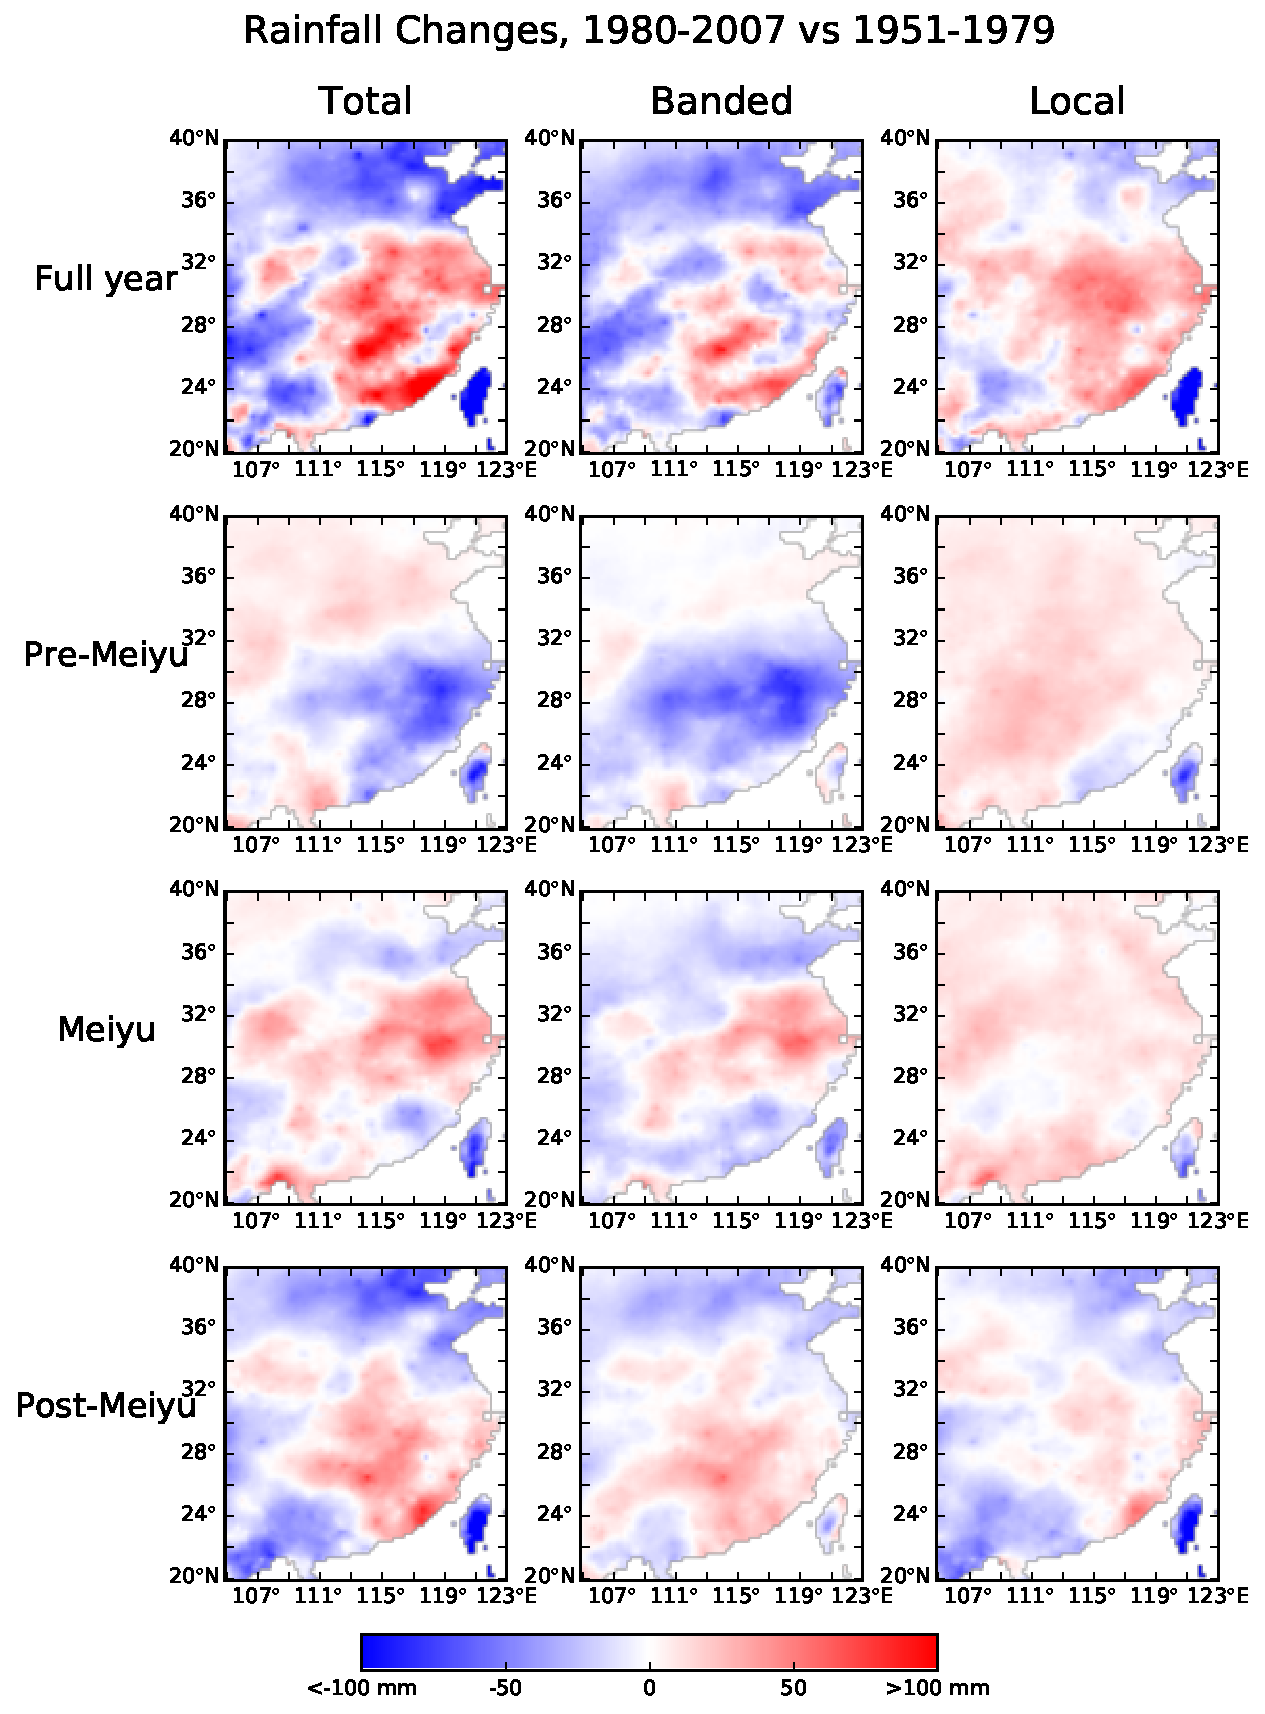
\includegraphics[width=\linewidth]{Figures/changes_by_type_8007_5179}
\caption{1980-2007 versus 1951-1979 changes in total, banded and local rainfall for full year, Pre-Meiyu (days 121-160), Meiyu (days 161-200) and Post-Meiyu (days 201-273), with significance at the 95\%/99\% level marked by single/double hatches (permutation test with 1,000 iterations). \textit{Banded} rainfall consists of all rainfall falling within 4$^{\circ}$ of a rainband axis and rainfall at any other adjacent point exceeding 10 mm day$^{-1}$. \textit{Local} rainfall includes all rainfall not meeting these criteria.}
\label{fig:type_decadal_8007_5179}
\end{figure}


%%FIGURE 5 Decadal changes in different rainfall types, 1994-2007 v 1980-1993
\begin{figure}[htb]
\centering
\noindent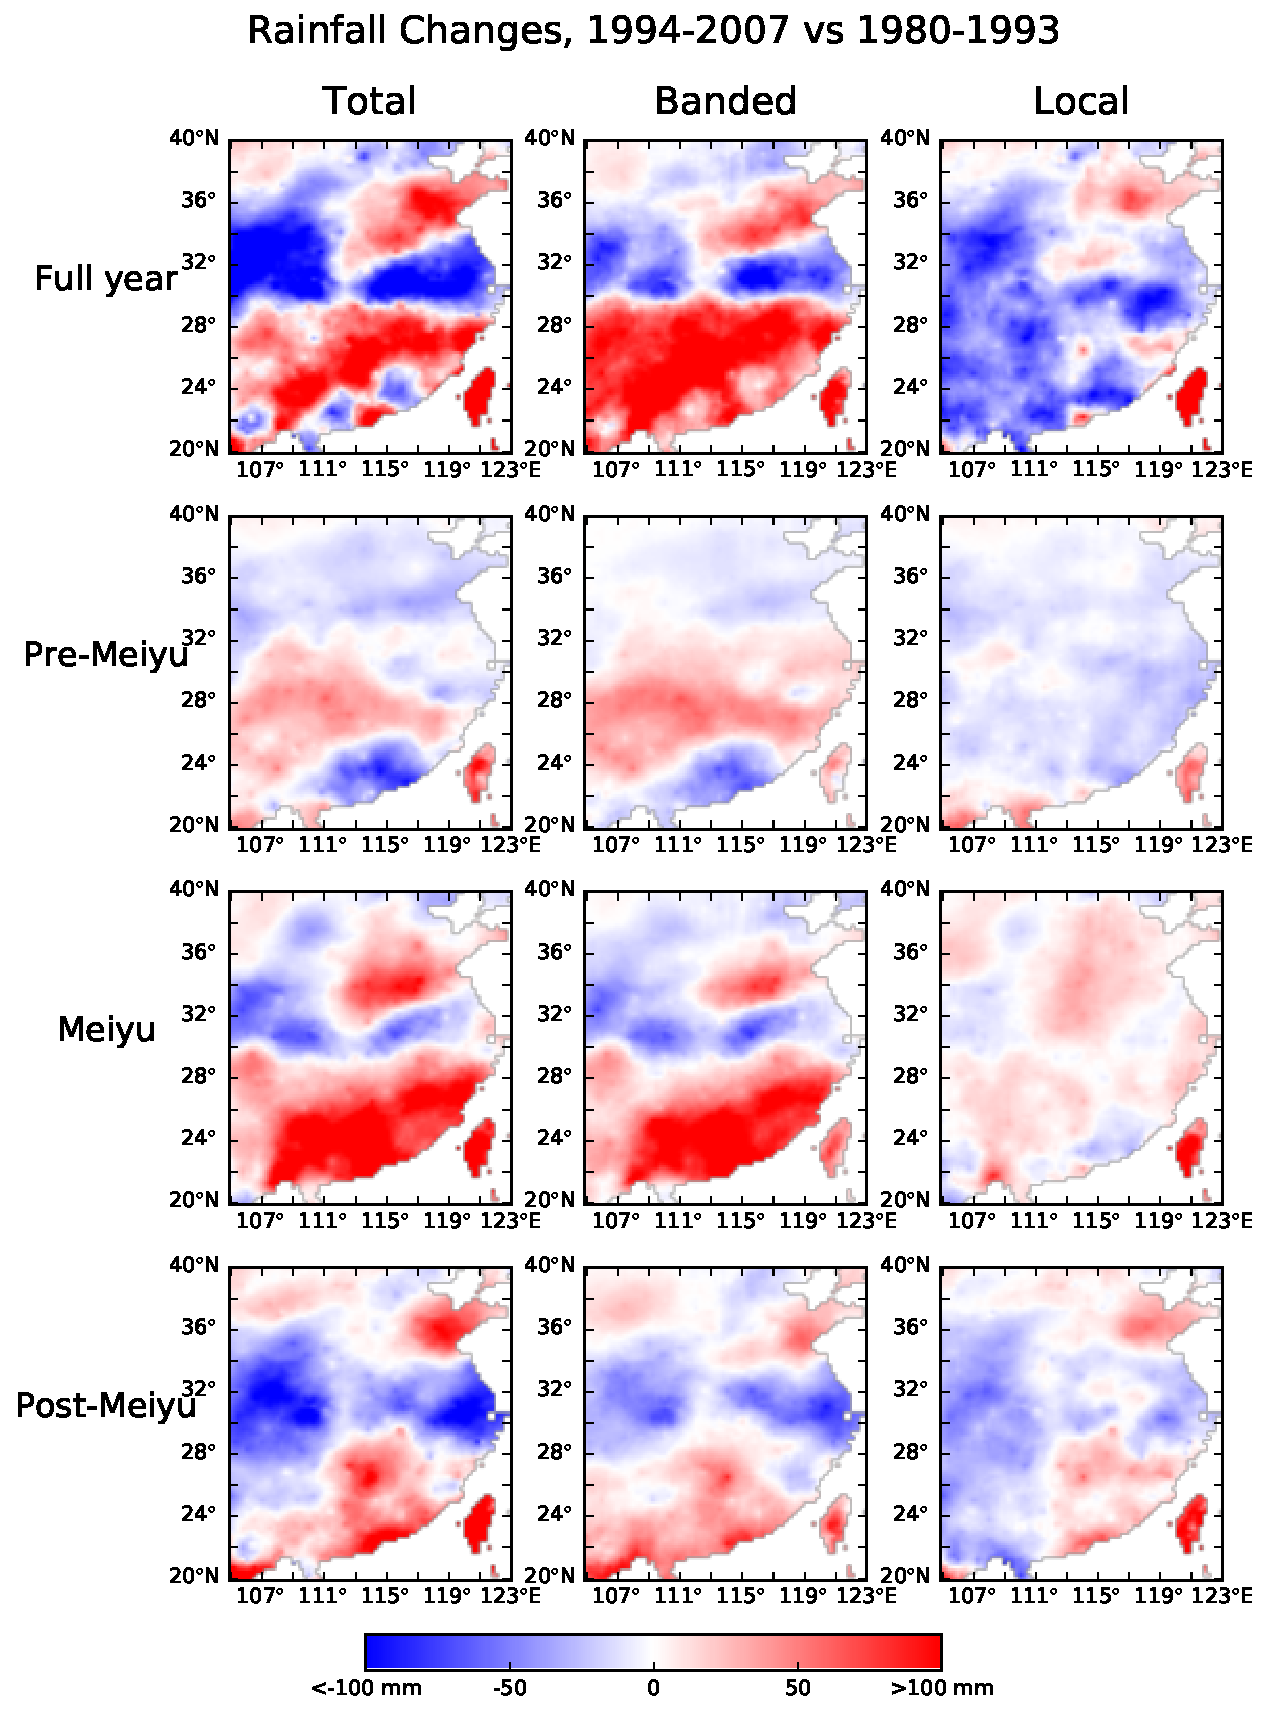
\includegraphics[width=\linewidth]{Figures/changes_by_type_9407_8093}
\caption{1980-2007 versus 1951-1979 changes in total, banded and local rainfall for full year, Pre-Meiyu (days 121-160), Meiyu (days 161-200) and Post-Meiyu (days 201-273), with significance at the 95\%/99\% level marked by single/double hatches (permutation test with 1,000 iterations). \textit{Banded} rainfall consists of all rainfall falling within 4$^{\circ}$ of a rainband axis and rainfall at any other adjacent point exceeding 10 mm day$^{-1}$. \textit{Local} rainfall includes all rainfall not meeting these criteria.}
\label{fig:type_decadal_9407_8093}
\end{figure}


%%FIGURE 3 Significance of attribute changes in rainbands between decades
\begin{figure}[htbp]
\centering
\noindent\includegraphics[width=\linewidth]{Figures/RDA_bars}
\caption{Significance of decadal changes in a) Rainband frequency, b) Rainband latitude and c) Rainband intensity between decades.}
\label{fig:bar}
\end{figure}

	
\subsection*{1980-1993 versus 1994-2007}
	
	We repeat the methodology described above with the set of years 1994-2007 versus 1980-1993, when past authors have reported a shift in South China rainfall \citep{Kwon2007,Wu2010,Yim2013}. Changes between these two time periods are shown in Figure~\ref{fig:sfnd}b. The spatial pattern of change during 1980-1993 versus 1994-2007 is distinct from that shown in 1980-2007 versus 1951-1979. Specifically, the former resembles a zonally symmetric tripole, whereas the latter resembles more of a dipole pattern. These are known to be the leading modes of eastern China rainfall variability \citep{Day2015}.
	
	Figure~\ref{fig:hov_9407_8093} shows that, unlike the 1980-2007 versus 1951-1979 comparison (Figure~\ref{fig:hov_8007_5179}), significant summer changes occur in both banded and local rainfall, especially in July and August. Figure~\ref{fig:hov_8007_5179} furthermore shows that rainbands have generally intensified year round, and especially during the pre-Meiyu and Meiyu seasons over southern China. In particular, during Meiyu season, mean rainband latitude shifted southward from $30.0^\circ \textrm{N} \pm .4^\circ$ to $28.9^\circ \textrm{N} \pm .4^\circ\ (p=.0002)$ and the \textit{intensity} of rainbands also jumped from $27.3 \pm 1.1$ mm day$^{-1}$ to $29.8 \pm 1.1$ mm day$^{-1}\ (p=.9994)$, leading to increased rainfall over central and southern China. \citet{Zou2015} also found that China experienced a more intense Meiyu during the 1990s, as well as generally more severe rainfall events. Unlike the comparison between 1951-1979 and 1980-2007, rainband \textit{frequency} remained unchanged. Testing for the significance of the change in distribution, both the KS and AD tests found an altered distribution of intensity and latitude of rainbands during Meiyu season during 1994-2007 relative to 1980-1993, with $p<.001$ for both changes \citet{Day2016}.
	
	In summary, the changes in rainfall between 1980-1993 and 1994-2007 are fundamentally different from the South Flood-North Drought pattern of changes between 1951-1979 and 1980-2007. In the former case, both banded and local rainfall experienced significant changes, and the change in banded rainfall was marked by a change in \textit{intensity}. During the latter, changes in the frequency of rainbands (without a change in intensity) led to decreases in banded rainfall. We propose that these two distinct kinds of decadal change reflect different forcing mechanisms, as explored in the conclusion.
	
	Other regions with distinct rainfall subclimates such as the Sichuan Basin and Taiwan have also undergone significant decadal changes in local rainfall independent from the rest of eastern China in which changes in local rainfall play an important role, further suggesting the utility of rainfall classification based on RDA.
	
%%FIGURE 6 Changes in rainfall by type between 1951-1979 and 1980-2007
\begin{figure}[htbp]
\centering
\noindent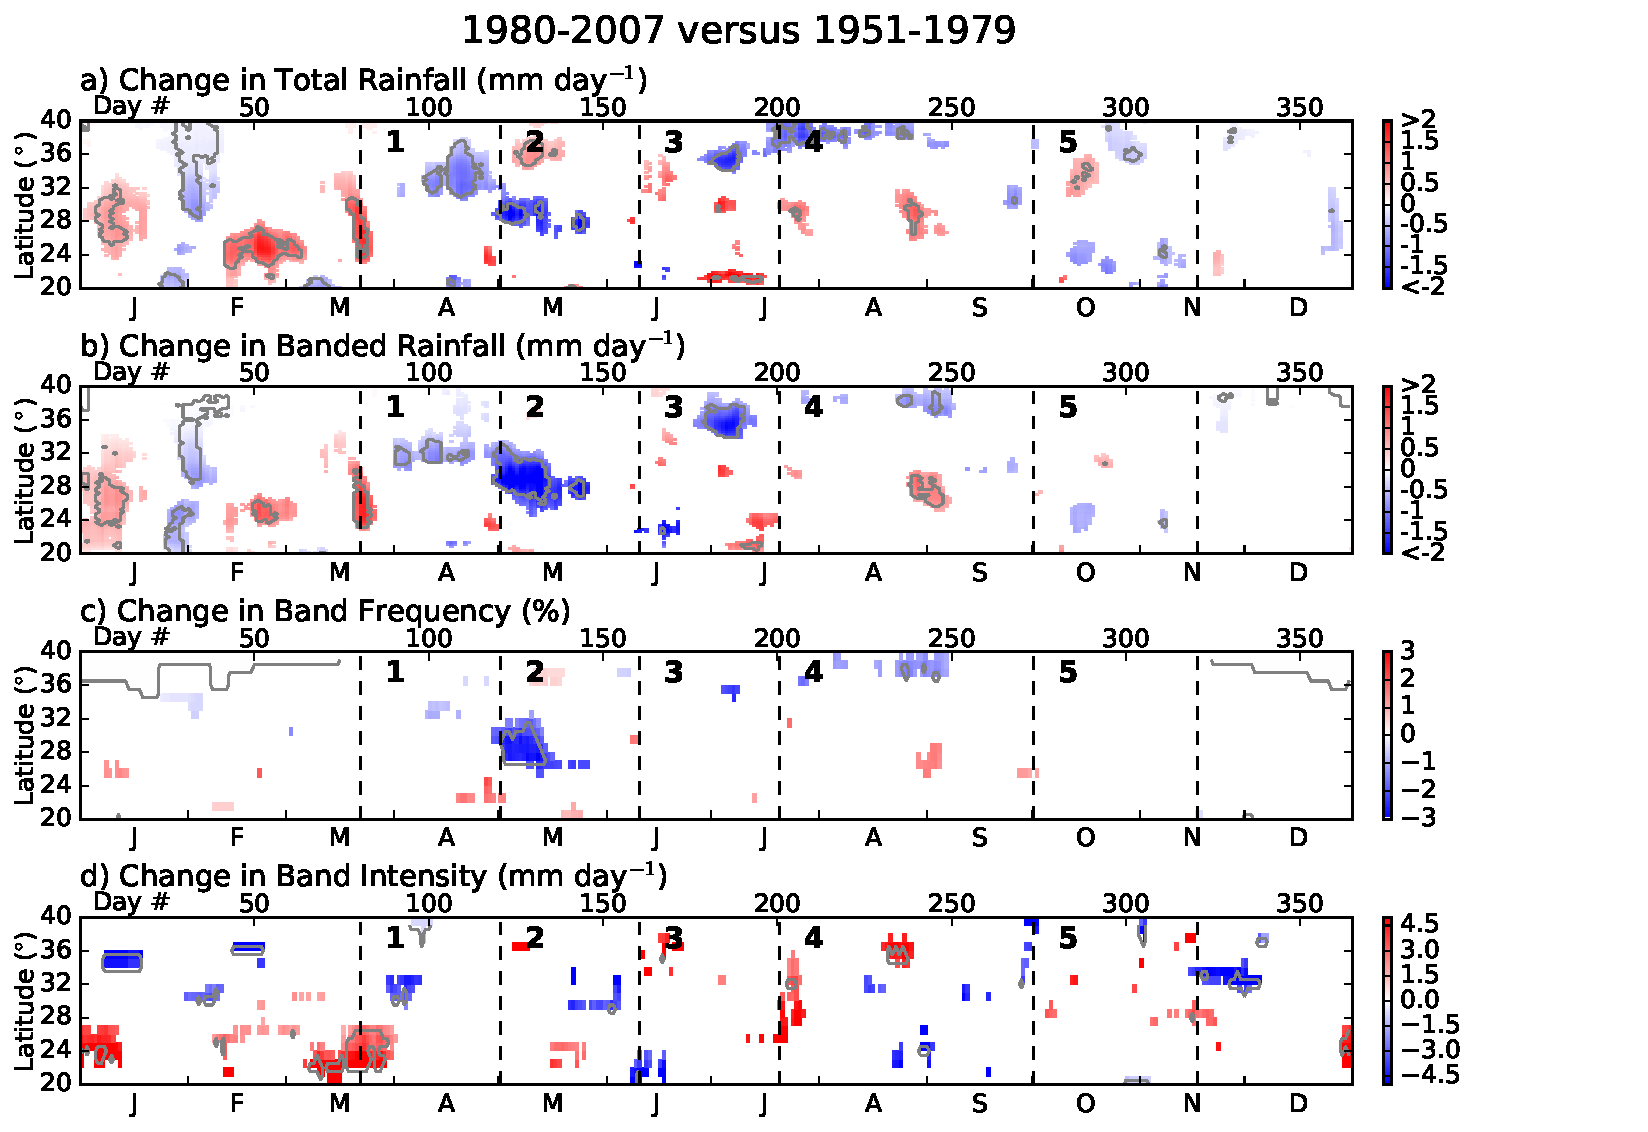
\includegraphics[width=\linewidth]{Figures/hov_summary_8007_5179}
\caption{15-day running mean of the change in a) total rainfall; b) banded rainfall; c) rainband frequency and d) rainband intensity between 1980-2007 and 1951-1979, zonally averaged by latitude over 110-123$^{\circ}$E. All changes shown are significant at a 95\% level, and significance exceeding a 99\% level is contoured in gray, as calculated by a moving blocks bootstrap with block length of 2 days and 2,000 iterations. Zonal rainfall averages \textit{exclude} rainfall occurring over Taiwan because the magnitude of changes over the island dwarf changes on the mainland.}
\label{fig:hov_8007_5179}
\end{figure}

%%FIGURE 7 Changes in rainfall by type between 1980-1993 and 1994-2007
\begin{figure}[htbp]
\centering
\noindent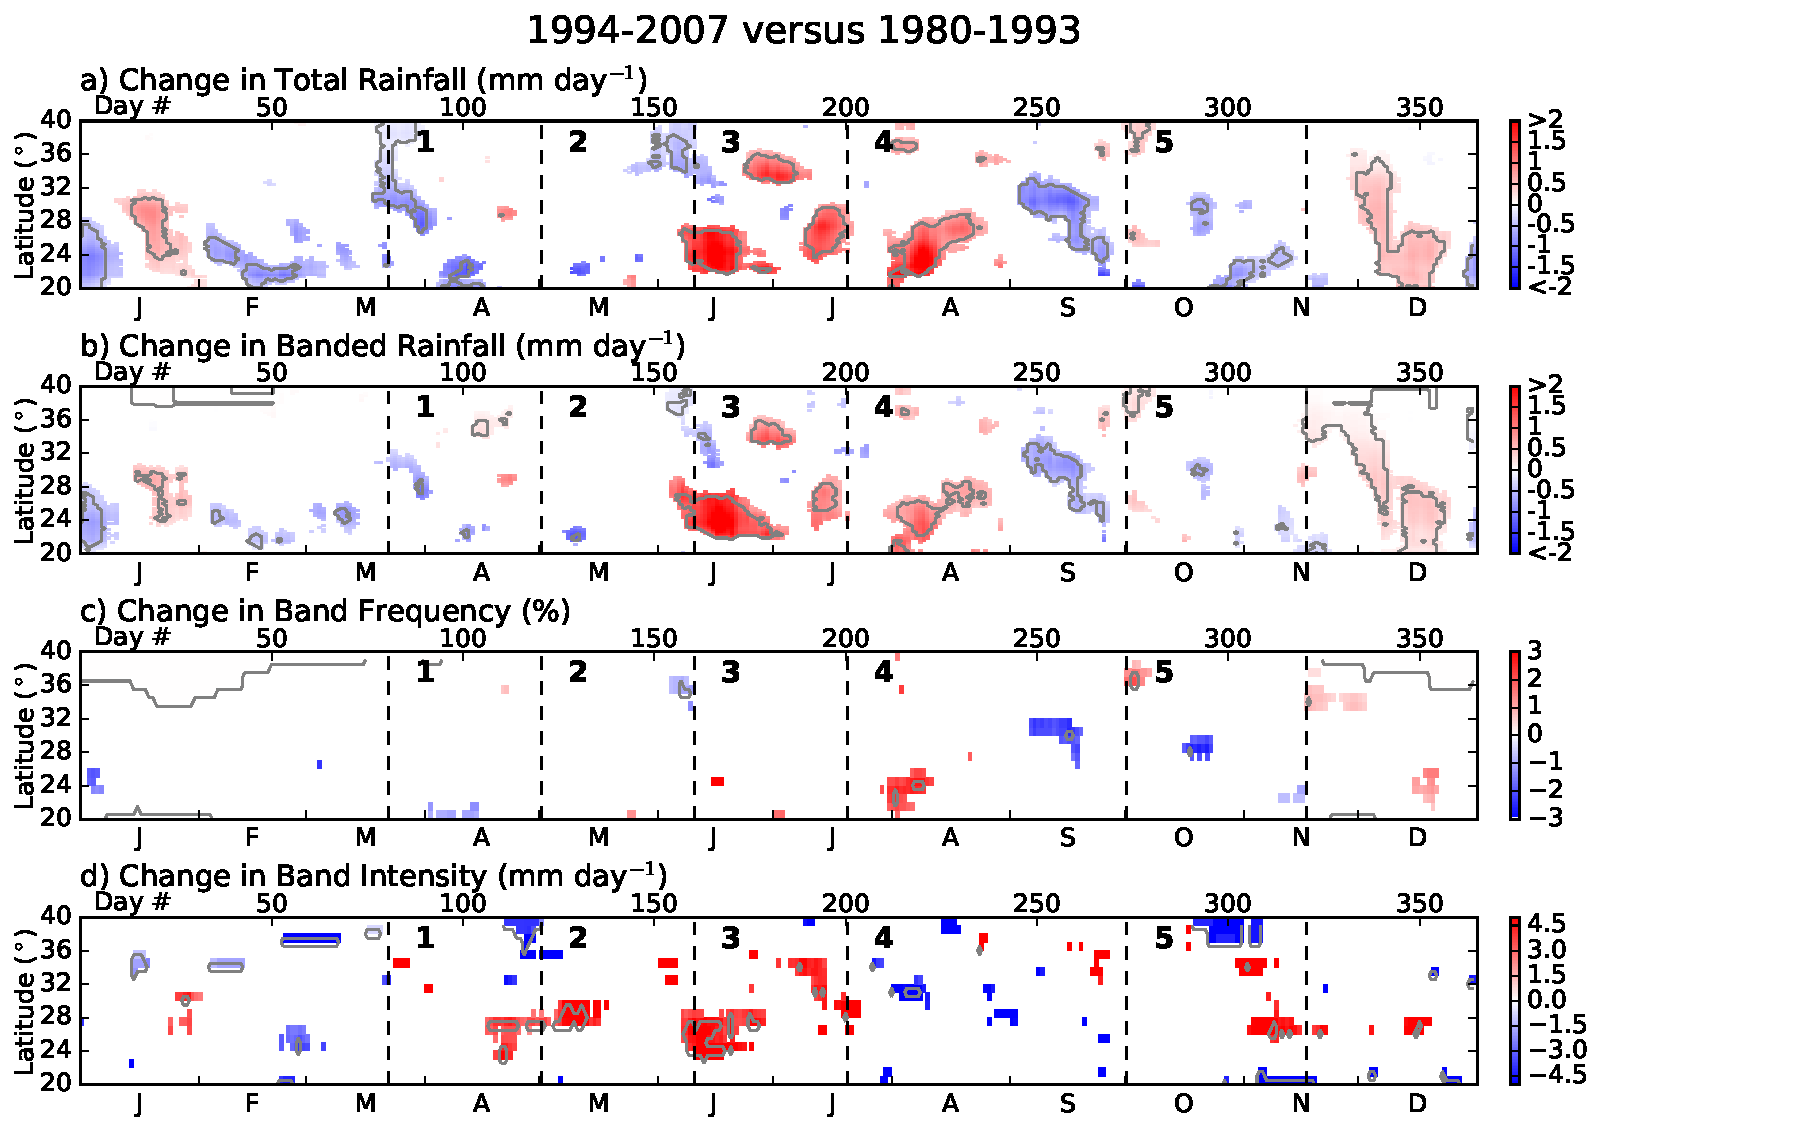
\includegraphics[width=\linewidth]{Figures/hov_summary_9407_8093}
\caption{15-day running mean of change in a) total rainfall; b) banded rainfall; c) rainband frequency and d) rainband intensity between 1994-2007 and 1980-93, zonally averaged by latitude over 110-123$^{\circ}$E. All changes shown are significant at a 95\% level and significance exceeding a 99\% level is contoured in gray, as calculated by a moving blocks bootstrap with block length of 2 days and 2,000 iterations. Zonal rainfall averages \textit{exclude} rainfall occurring over Taiwan because the magnitude of changes over the island dwarf changes on the mainland.}
\label{fig:hov_9407_8093}
\end{figure}
	
\section*{Conclusion}

	This work has aimed to quantify the role of frontal storms in the yearly rainfall climatology of eastern China. We used the Rainband Detection Algorithm (RDA), a recursive image processing algorithm, to compile a 57-year catalog of daily rainband occurrence over China and the properties of each event, such as latitude, intensity, tilt, width and length. Over 50\% of yearly total precipitation is contributed by banded rainfall in most of eastern China. We identify a sequence of 5 stages of frontal precipitation, each with preferred position, frequency and strength of frontal rainfall: 1) the Spring Rains (March 1-April 30); 2) the Pre-Meiyu (May 1-June 9); 3) the Meiyu (June 10-July 19); 4) the Post-Meiyu (July 20-September 30) and 5) the Fall Rains (October 1-November 16) (Figure~\ref{fig:hov}). The climatological transitions from one period to the next are marked by sharp changes in rainband frequency, latitude and intensity. Simpler alternative metrics of eastern China rainfall fail to reproduce most of these features.
	
	Our product makes no assumptions about the causative mechanisms of eastern China rainfall. The fact that bands of rainfall spanning over 10$^{\circ}$ in longitude occur at all times of year suggests a consistent mechanism of formation, and also that the classification between banded and local rainfall effectively distinguishes between large-scale convergence and other mechanisms with shorter length scale such as local convection and orographic triggering. This is further supported by the distinct seasonality of banded and local rainfall: The former peaks during Meiyu season (late June), while the latter peaks during the Post-Meiyu (early August).
	
	Decadal changes in rainfall in eastern China are mostly due to changes in banded rainfall, as opposed to local rainfall (Figures~\ref{fig:type_decadal_8007_5179} and~\ref{fig:type_decadal_9407_8093}). The use of RDA allows us to further attribute changes either to altered rainband frequency or intensity. Over the full 57-year period, a decrease in northern China rainband \textit{frequency} was the principal contributor to late-\nth{20}-century drought (Figure~\ref{fig:hov_8007_5179}), as revealed by a southward shift in Post-Meiyu mean rainband latitude with $p=<.001$. The start of the rainy season over the Yangtze Valley was also postponed due to a decline in rainband frequency ($p=0.02$). In contrast, a comparison of 1994-2007 versus 1980-1993 reveals an uptick in rainband \textit{intensity} during Meiyu season with no change in frequency (Figure~\ref{fig:hov_9407_8093}; $p>.999$). The magnitude of these signals suggests that they are not merely an artifact of natural variability.
	 
	 Potential causes of altered rainfall include global and regional-scale forcing. The changing nature of rainfall may serve as fingerprint of the predominance of a particular forcing on a given time scale . On a paleo-climatic time scale, \citet{Chiang2015} argued for joint modulation between the seasonal cycle of the East Asian jet and East Asian rainfall. The annual progression of the Meiyu front and anomalous shifts both entail large-scale circulation anomalies \citep{Chen2004,Kosaka2011}. During the second half of the \nth{20} century, a southward trend in the latitude of the East Asian tropospheric jet latitude has been observed, attributed to global warming \citep{Yu2007, Archer2008,Park2014a}. Causality cannot be proved from the observations (the shift in East Asian jet latitude may be a response to rainfall changes), 
	 
A potential culprit are the aerosols produced during the late-twentieth-century industrialization and urbanization of East China, which have had a substantial impact on atmospheric temperature and cloud properties across Asia \citep{Menon2002,Fan2012,Streets2013}. \citet{Choi2008} found that, on a daily scale, the concentration of PM10 aerosols (diameter less than 10 $\mu m$) is positively correlated with medium-to-heavy rainfall and negatively correlated with the occurrence of light rainfall. In addition, a modeling study by \citet{Wang2016} suggests that the largest impact on eastern China rainfall has come from the effect of aerosols on cloud microphysics, leading to a shift toward more intense precipitation. Thus, changes in aerosol concentration can explain an increase in rainfall intensity without an increase in its frequency.
	
 Some studies attribute the South Flood-North Drought to natural variability \citep{Zhang1999,Xin2006,Lei2014}, but \citet{Zhou2009} claimed that the South Flood-North Drought was distinct from other patterns of \nth{20}-century variability. The East Asian jet is projected to continue shifting southward in the \nth{21} century due to the influence of continued global warming \citep{Park2014}. We propose that this shift will cause a further decrease in the frequency of northern China banded rainfall, potentially intensifying the South Flood-North Drought pattern. In contrast, the concentration of anthropogenic aerosols is projected to decline during the \nth{21} century \citep{Westervelt2015}, and so we expect the intensity of rainbands and local rainfall to both return to their 1951-1993 baseline. global mean surface temperature \citep{Zhao2010},.
	
	It is essential to understand whether the South Flood-North Drought pattern will persist under \nth{21}-century warming \citep{Zhang1999,Xin2006,Lei2014}. The CMIP5 (Climate Model Intercomparison Project) model suite contained in the Intergovernmental Panel on Climate Change's Fifth Assessment Report (IPCC AR5) does not agree on the sign of future summer rainfall changes in East Asia \citep{Christensen2011}.Depending on whether global warming or aerosols are implicated, we might expect late \nth{20}-century trends to be further exacerbated, or instead to return to their \nth{20} century baseline.
 Other authors have suggested changes in Indian Ocean SST \citep{Qu2012}, decreased sensible heating from the Tibetan Plateau \citep{Liu2012a,Hu2015} and aerosol forcing \citep{Song2014} as culprit.

Figure \ref{fig:frog} shows an example of how to insert a column-wide figure. To insert a figure wider than one column, please use the \verb|\begin{figure*}...\end{figure*}| environment. Figures wider than one column should be sized to 11.4 cm or 17.8 cm wide.

%\begin{table}%[tbhp]
%\centering
%\caption{Comparison of the fitted potential energy surfaces and ab initio benchmark electronic energy calculations}
%\begin{tabular}{lrrr}
%Species & CBS & CV & G3 \\
%\midrule
%1. Acetaldehyde & 0.0 & 0.0 & 0.0 \\
%2. Vinyl alcohol & 9.1 & 9.6 & 13.5 \\
%3. Hydroxyethylidene & 50.8 & 51.2 & 54.0\\
%\bottomrule
%\end{tabular}

%\addtabletext{nomenclature for the TSs refers to the numbered species in the table.}
%\end{table}

\subsection*{Supporting Information (SI)}

\subsection{Alternative Metrics of China Rainfall}

Since the RDA method is complex, we must justify its use by proving that it supplies information about China rainfall beyond what simpler metrics can provide. We define a suite of potential daily rainfall metrics as follows: 

\begin{itemize}

	\item $M_1$ - Latitude of maximum rainfall;
	
	\item $M_2$ - Intensity-weighted centroid of daily rainfall latitude;
	
	\item $M_3$ - Intensity of maximum rainfall over China (100-123$^{\circ}$E and 20-40$^{\circ}$N);
	
	\item $M_4$ - Area-averaged intensity of China rainfall; 
	
	\item $M_5$ - Area-averaged intensity of North China rainfall (107.5-125$^{\circ}$E and 37-42$^{\circ}$N); 
	
	\item $M_6$ - Area-averaged intensity of South China rainfall (107.5-122.5$^{\circ}$E and 27-33$^{\circ}$N); 
	
	\item $M_7$ - \% of days where $M_5$ exceeds 1 mm day$^{-1}$ (\textit{frequency} of North China rainfall);
	
	\item $M_8$ - \% of days where $M_6$ exceeds 1 mm day$^{-1}$ (\textit{frequency} of South China rainfall).
	
\end{itemize}

 The definitions of the North China and South China regions are the same as in \citet{Yu2010}. A full year climatology of each metric during different time periods is presented in Figure~\ref{fig:alternative_metrics}. Mean values during different seasons are listed in \citet{Day2016}. Where applicable, the significance of change was calculated including the autocorrelation of each metric. In general, the changes in these metrics are fewer and less discernible than those revealed by the use of RDA.
 
 \subsection{Temporal Autocorrelation}

	Fronts and rainbands tend to persist for several days. Therefore, rainfall amounts and front attributes on successive days are not fully independent observations, which reduces the effective number of degrees of freedom of these time series. This temporal autocorrelation must be accounted for in calculations of statistical significance such as estimating the $p$-value of a change in rainband frequency between two time periods. In this particular case, we use the analytic formula for a Bernoulli process (applicable for any time series where observations are binary) with effective number of degrees of freedom $n=\frac{N}{\tau}$ for number of days $N$ and decorrelation time $\tau$ given by

\begin{equation*}
\tau=1+2\sum_{k=1}^m \rho(k)
\end{equation*}

	where $\rho(k)$ is the autocorrelation function of rainband existence with lag $k$ \citep{VonStorch1999}. We calculate $\tau$ using a maximum lag of $m=10$ days. The yearly mean decorrelation timescale of rainband frequency is found to be $\tau = 1.81$ after removing the seasonal cycle. This value is used to calculate significance of changes in Figure 3b. The standard deviation and $p$-values of rainband frequency shown in Figure~\ref{fig:bar} use seasonal values of $\tau$ shown in \citet{Day2016}. $\tau$ is also used to select block length for moving blocks bootstrap tests, as described below.
 
\subsection{Significance of Changes}

\subsubsection{Bootstrapping with and without Replacement}

	Observations of rainband latitude and intensity during a given time period obey unknown distributions. Therefore, we require non-parametric tests to estimate the standard deviation of their mean and the significance of changes in mean. We employ bootstrapping with and without replacement (the latter also known as a permutation test), well-established techniques that estimate quantities of interest by constructing synthetic distributions with random sampling of original data \citep{Good2005}. We calculate the significance of changes in mean rainband latitude and intensity between 1951-1979 and 1980-2007, and also repeat our methodology for 1980-1993 versus 1994-2007 (Figure~\ref{fig:bar}).

\subsubsection{Moving Blocks Bootstrap}	
	
	The bootstrap must be adapted for time series featuring temporal autocorrelation. In such time series, a single anomalous weather event will persist over several days, and a bootstrap method will tend to exaggerate the significance of differences between the two original distributions. To avoid this scenario, we use a \textit{moving blocks bootstrap} test, described for instance in \citet{Singh2014}. This technique is identical to bootstrapping with replacement except that samples are drawn in continuous blocks of length $n$ that preserve the time structure of the original data set. Block length is chosen based on decorrelation time scale $\tau$. The autocorrelation of daily rainfall in China is approximately $\tau =2-3$ days, and therefore the significance estimates in Figure~\ref{fig:hov}a use a moving blocks bootstrap with block length of 2 days and 2000 iterations. In general, a choice of block lengths between 2 and 5 days leads to similar results. Our MATLAB code for the permutation test and the moving blocks bootstrap is included in the appendix.
	
\subsection{Significance of Changes in Distribution}

	A moving blocks bootstrap cannot be used for time series with gaps. However, using a permutation test to estimate the significance of changes in the mean of latitude and intensity may overestimate their significance. Therefore, we verify results by also implementing a Kolmogorov-Smirnov (K-S) and Anderson-Darling (A-D) tests, each of which estimates the probability that two samples were drawn from the same distribution. Both the K-S and A-D tests define a test statistic based on the largest difference between the observed probability distribution of two samples. Similar to a $t$-test, the value of this test statistic can be translated into a $p$-value. We first define the \textit{empirical distribution function} $F_1(x)$ and $F_2(x)$ of each sample. All $n$ observations in each sample are ordered as $\left\{X_1 < ... < X_n\right\}$, after which $F(x)$ is calculated as follows:

\begin{align}
	F(x) =& \frac{1}{n}\sum_{i=1}^n I_{[-\infty,x]} (X_i) \\
	I_{[-\infty,x]} =& 
	\begin{cases}
   		 1 & \text{if } X_i \leq x\\
    		0 & \text{otherwise} \\
    	\end{cases}
\end{align}

 The K-S test statistic $D$ is then defined as the maximal distance between the two empirical distribution functions:

\begin{equation}
	D=\max_{all\ x} |F_{1}(x)-F_{2}(x)|
\end{equation}

$D$ can then be inverted to derive a $p$-value. The Anderson-Darling (A-D) test statistic $A^2$ resembles $D$, but is formulated to be more sensitive to the tails of the distribution:

\begin{equation}
	A^2 = -n-S \,,
	\mathrm{where}
\end{equation}

\begin{equation}
	S=\sum_{i=1}^n \frac{2i-1}{n}\left[\ln(F(X_i)) + \ln\left(1-F(X_{n+1-i})\right)\right].
\end{equation}

	$A^2$ can likewise be translated into a $p$-value. The K-S and A-D tests cannot be used if values are repeated within samples, because $D$ and $A^2$ are then undefined. We solve this problem by using bootstrap versions of these tests. Bootstrap K-S and A-D tests were performed as tests in R with 10,000 iterations. The significance of changes in the distribution of rainband latitude and intensity were previously presented in \citet{Day2016}. Both tests produce fairly similar results.

\subsubsection*{SI Text}

Supply Word, RTF, or LaTeX files (LaTeX files must be accompanied by a PDF with the same file name for visual reference).

\subsubsection*{SI Figures}

Provide a brief legend for each supporting figure after the supporting text. Provide figure images in TIFF, EPS, high-resolution PDF, JPEG, or GIF format; figures may not be embedded in manuscript text. When saving TIFF files, use only LZW compression; do not use JPEG compression. Do not save figure numbers, legends, or author names as part of the image. Composite figures must be pre-assembled.

\subsubsection*{SI Tables}

Supply Word, RTF, or LaTeX files (LaTeX files must be accompanied by a PDF with the same file name for visual reference); include only one table per file. Do not use tabs or spaces to separate columns in Word tables.

\subsubsection*{Appendices}

PNAS prefers that authors submit individual source files to ensure readability. If this is not possible, supply a single PDF file that contains all of the SI associated with the paper. This file type will be published in raw format and will not be edited or composed.

\matmethods{
\subsection*{APHRODITE Rainfall}

	The APHRO\_MA\_V1101 product from APHRODITE (Asian Precipitation - Highly-Resolved Observational Data Integration Towards Evaluation of the Water Resources) includes 57 years (1951-2007) of continental daily rainfall (PRECIP product) on a .25$^{\circ} \times .25^{\circ}$ grid over 60$^{\circ}$-150$^{\circ}$E and 15$^{\circ}$S-55$^{\circ}$N \citep{Yatagai2012}, as well as a daily map of reporting weather stations on the same grid (RSTN product). Values are reported over land only. We focus on the subregion inside of 105$^{\circ}$E-123$^{\circ}$E and 20$^{\circ}$N-40$^{\circ}$N where rainbands are known to occur frequently, especially during Meiyu season (early June to late July). The network of stations remains dense (100-200 km spacing) through time, such that rainbands are clearly resolved and we are not concerned about potential artifacts from changes in station density. APHRODITE's resolution cannot capture some features visible in TRMM satellite data \citep{Xu2009}, but its length allows for the study of decadal change. We use the words ``rainfall'' and ``precipitation'' interchangeably in the rest of this work since most precipitation consists of rain, although snow is common in northeastern China during winter.
}

\showmatmethods % Display the Materials and Methods section

\acknow{	APHRODITE precipitation data is publicly available at \url{http://www.chikyu.ac.jp/precip/index.html}. The rainband detection algorithm was written in MATLAB and data analysis carried out with Jupyter Notebook. The author's data analysis is freely available on Github. Ferret, a NOAA product, was used for some figure generation and is freely available at \url{http://ferret.pmel.noaa.gov/Ferret/}. A full database of rainband statistics from 1 January 1951 to 31 December 2007 and associated MATLAB and Ferret codes used to produce results are available on the author's Github repository. This work was supported by NSF grants EAR-0909195 and EAR-1211925, which allowed the presentation of preliminary results in conference settings and the feedback of our peers, as well as DOE grant DE-SC0014078. We also acknowledge NSFC (National Natural Science Foundation of China) grant \#40921120406 for enabling our collaboration with Professor Yanjun Cai of IEECAS in Xi'an, which led to the present work. We thank Jinqiang Chen and an anonymous reviewer for valuable suggestions on a previous version of this manuscript.}

\showacknow % Display the acknowledgments section

% \pnasbreak splits and balances the columns before the references.
% If you see unexpected formatting errors, try commenting out this line
% as it can run into problems with floats and footnotes on the final page.
\pnasbreak

% Bibliography
\bibliography{RDA_biblio}

\end{document}